\documentclass[aspectratio=169,10pt]{beamer}

\usetheme{default}

\usepackage[T1]{fontenc}
\usepackage[utf8]{inputenc}
\usepackage[english]{babel}
\usepackage{amsmath,amssymb,amsfonts}
\usepackage{array}
\usepackage{booktabs}
\usepackage{graphicx}
\usepackage{tikz}
\usetikzlibrary{arrows.meta,positioning}
\usepackage{appendixnumberbeamer}
\usepackage[babel,english=american]{csquotes}
\usepackage[backend=biber,style=ieee,isbn=false,sortcites,maxbibnames=6,minbibnames=1]{biblatex}

\definecolor{azulUC3M}{RGB}{0,0,102}
\definecolor{uc3mLight}{RGB}{232,236,247}
\definecolor{annGreen}{RGB}{22,119,84}
\definecolor{pinnOrange}{RGB}{191,91,36}
\definecolor{refBlue}{RGB}{35,80,150}
\definecolor{gray45}{gray}{.45}
\definecolor{gray95}{gray}{.95}

\setbeamersize{text margin left=8mm,text margin right=8mm}
\setbeamercolor{structure}{fg=azulUC3M}
\setbeamercolor{title}{fg=azulUC3M}
\setbeamercolor{frametitle}{fg=azulUC3M}
\setbeamerfont{frametitle}{size=\Large,series=\bfseries}
\setbeamerfont{title}{size=\Large,series=\bfseries}
\setbeamerfont{subtitle}{size=\normalsize}
\setbeamercolor{section in toc}{fg=azulUC3M}
\setbeamercolor{block title}{bg=azulUC3M,fg=white}
\setbeamercolor{block body}{bg=gray95,fg=black}
\setbeamertemplate{itemize item}{\color{azulUC3M}\small$\blacktriangleright$}
\setbeamertemplate{itemize subitem}{\color{azulUC3M}\scriptsize$\bullet$}
\setbeamertemplate{navigation symbols}{}
\setbeamertemplate{headline}{}
\setbeamertemplate{footline}{%
  \leavevmode%
  \begin{beamercolorbox}[wd=\paperwidth,ht=2.5ex,dp=1.2ex,rightskip=8mm plus1fil]{date in head/foot}%
    \hfill\color{gray45}\insertframenumber/\inserttotalframenumber
  \end{beamercolorbox}%
  \vskip0pt%
}

\setbeamertemplate{title page}{%
  \vspace{3mm}
  \begin{flushleft}
    {\usebeamerfont{title}\usebeamercolor[fg]{title}\inserttitle\par}
    \vspace{2mm}
    {\usebeamerfont{subtitle}\insertsubtitle\par}
    \vspace{7mm}
    {\usebeamerfont{author}\insertauthor\par}
    \vspace{3mm}
    {\usebeamerfont{institute}\insertinstitute\par}
    \vspace{5mm}
    {\usebeamerfont{date}\insertdate\par}
  \end{flushleft}
}

\graphicspath{{figures/}{../figures/}}
\addbibresource{../references.bib}

\title[TFM Defense]{Physics-Informed and Data-Driven Neural Networks for Option Pricing, Calibration, and Greeks Estimation under the Heston Model}
\subtitle{Master Thesis Defense}
\author[J. E. Zafra Mena]{Jose Enrique Zafra Mena}
\institute[UC3M]{Master Degree in Applied and Computational Mathematics\\Universidad Carlos III de Madrid\\[3mm]\textbf{Supervisors:}\\Jorge Morón Vidal\\Francisco Manuel Bernal Martínez}
\date{Madrid, 2026}

\newcommand{\metric}[2]{\begin{tabular}{@{}c@{}}{\Large\bfseries #1}\\[-1mm]{\scriptsize #2}\end{tabular}}

\newcommand{\workflowdiagram}[2]{%
\begin{tikzpicture}[
  font=\scriptsize,
  box/.style={draw, rounded corners=2pt, align=center, minimum height=0.62cm, text width=1.55cm, inner sep=2.5pt, line width=0.35pt},
  refbox/.style={box, fill=refBlue!10, draw=refBlue!75},
  nnbox/.style={box, fill=annGreen!11, draw=annGreen!75, opacity=#1, text opacity=#1},
  pinnbox/.style={box, fill=pinnOrange!13, draw=pinnOrange!80, opacity=#2, text opacity=#2},
  outbox/.style={box, fill=gray95, draw=gray45!60},
  arrow/.style={-{Latex[length=2.1mm,width=1.5mm]}, line width=0.45pt, draw=black!70},
  annarrow/.style={arrow, draw=annGreen!80, opacity=#1},
  pinnarrow/.style={arrow, draw=pinnOrange!80, opacity=#2},
  greekline/.style={line width=0.55pt, dash pattern=on 2.5pt off 1.8pt, draw=azulUC3M!70}
]
  \node[refbox] (setup) at (0.0,0.0) {Heston\\contracts};
  \node[refbox] (cos) at (2.2,0.0) {COS\\pricing};
  \node[refbox] (iv) at (4.4,0.0) {IV\\inversion};
  \node[refbox] (refs) at (6.6,0.0) {Reference\\Greeks};

  \node[nnbox] (annbase) at (2.2,-1.35) {ANN\\baseline};
  \node[nnbox] (annsobo) at (4.4,-1.35) {ANN\\Sobolev};
  \node[nnbox] (cann) at (6.6,-1.35) {CaNN\\calibration};
  \node[outbox, opacity=#1, text opacity=#1] (anngreeks) at (8.9,-1.35) {ANN/CaNN\\diagnostics};

  \node[pinnbox] (pinnbase) at (2.2,-2.85) {PINN\\baseline};
  \node[pinnbox] (pinnsobo) at (4.4,-2.85) {PINN\\Sobolev};
  \node[pinnbox] (pinnacv) at (6.6,-2.85) {PINN Sobolev\\+ ACV};
  \node[outbox, opacity=#2, text opacity=#2] (pinngreeks) at (8.9,-2.85) {Pricing / Greek\\diagnostics};

  \draw[arrow] (setup) -- (cos);
  \draw[arrow] (cos) -- (iv);
  \draw[arrow] (iv) -- (refs);
  \draw[annarrow] (iv.south) -- ++(0,-0.37) -| (annbase.north);
  \draw[annarrow] (annbase) -- (annsobo);
  \draw[annarrow] (annsobo) -- (cann);
  \draw[annarrow] (cann) -- (anngreeks);
  \draw[pinnarrow] (setup.south) |- (pinnbase.west);
  \draw[pinnarrow] (pinnbase) -- (pinnsobo);
  \draw[pinnarrow] (pinnsobo) -- (pinnacv);
  \draw[pinnarrow] (pinnacv) -- (pinngreeks);
  \draw[greekline] (refs.south) -- (5.45,-0.78);
  \draw[greekline, -{Latex[length=2.1mm,width=1.5mm]}, opacity=#1] (5.45,-0.78) -- (annsobo.north);
  \draw[greekline, opacity=#2] (5.45,-0.78) -- (5.45,-2.28);
  \draw[greekline, -{Latex[length=2.1mm,width=1.5mm]}, opacity=#2] (5.45,-2.28) -- (pinnsobo.north);
\end{tikzpicture}%
}

\begin{document}

\begin{frame}[plain]
  \titlepage
  \vspace{-4mm}
  \centering
  
\includegraphics[width=0.28\linewidth]{logo_UC3M.png}
\end{frame}

\section{Context and Motivation}

\begin{frame}{Problem setting}
  \begin{block}{Placeholder claim}
    State why fast and accurate derivative pricing matters for calibration, risk, and model analysis under stochastic volatility models such as Heston \cite{heston}.
  \end{block}

  \begin{itemize}
    \item Introduce the target pricing problem and market context.
    \item Explain the computational bottleneck in repeated option valuation.
    \item Connect the problem to the thesis scope and evaluation criteria.
  \end{itemize}
\end{frame}

\begin{frame}{Research objectives}
  \begin{itemize}
    \item Objective 1: describe the baseline numerical pricing method.
    \item Objective 2: build and evaluate neural surrogate models.
    \item Objective 3: study calibration and Greek consistency.
    \item Objective 4: compare accuracy, speed, and robustness.
  \end{itemize}
\end{frame}

\section{Methodology}

\begin{frame}{Methodological pipeline}
  \begin{enumerate}
    \item Generate or collect option data under the selected volatility model.
    \item Price options with the numerical benchmark.
    \item Train surrogate models on controlled parameter domains.
    \item Evaluate prices, implied volatilities, calibration, and Greeks.
  \end{enumerate}
\end{frame}

\begin{frame}{Models and algorithms}
  \begin{columns}[T,onlytextwidth]
    \begin{column}{0.48\textwidth}
      \begin{block}{Numerical benchmark}
        Placeholder for COS method \cite{fang_oosterlee_2009}, Black-Scholes utilities, and implied volatility inversion.
      \end{block}
    \end{column}
    \begin{column}{0.48\textwidth}
      \begin{block}{Learning-based components}
        Placeholder for ANN surrogate, CaNN calibration \cite{liu}, PINN losses, and Greek adapters.
      \end{block}
    \end{column}
  \end{columns}
\end{frame}

\section{Results}

\begin{frame}{The ANN baseline gives a stable IV surrogate}
  \begin{columns}[T,onlytextwidth]
    \begin{column}{0.67\textwidth}
      \centering
      
\includegraphics[width=\linewidth,height=0.78\textheight,keepaspectratio]{nn/sensitivity_grid_3x2_log.png}
    \end{column}
    \begin{column}{0.29\textwidth}
      \begin{itemize}
        \item Test IV RMSE:
        \[
          1.86\cdot 10^{-3}.
        \]
        \item Stable behaviour in the interpolation core.
        \item Error increases near boundary and extrapolation regions.
      \end{itemize}
    \end{column}
  \end{columns}
\end{frame}

\begin{frame}{Sobolev training concentrates ANN Greek errors}
  \centering
  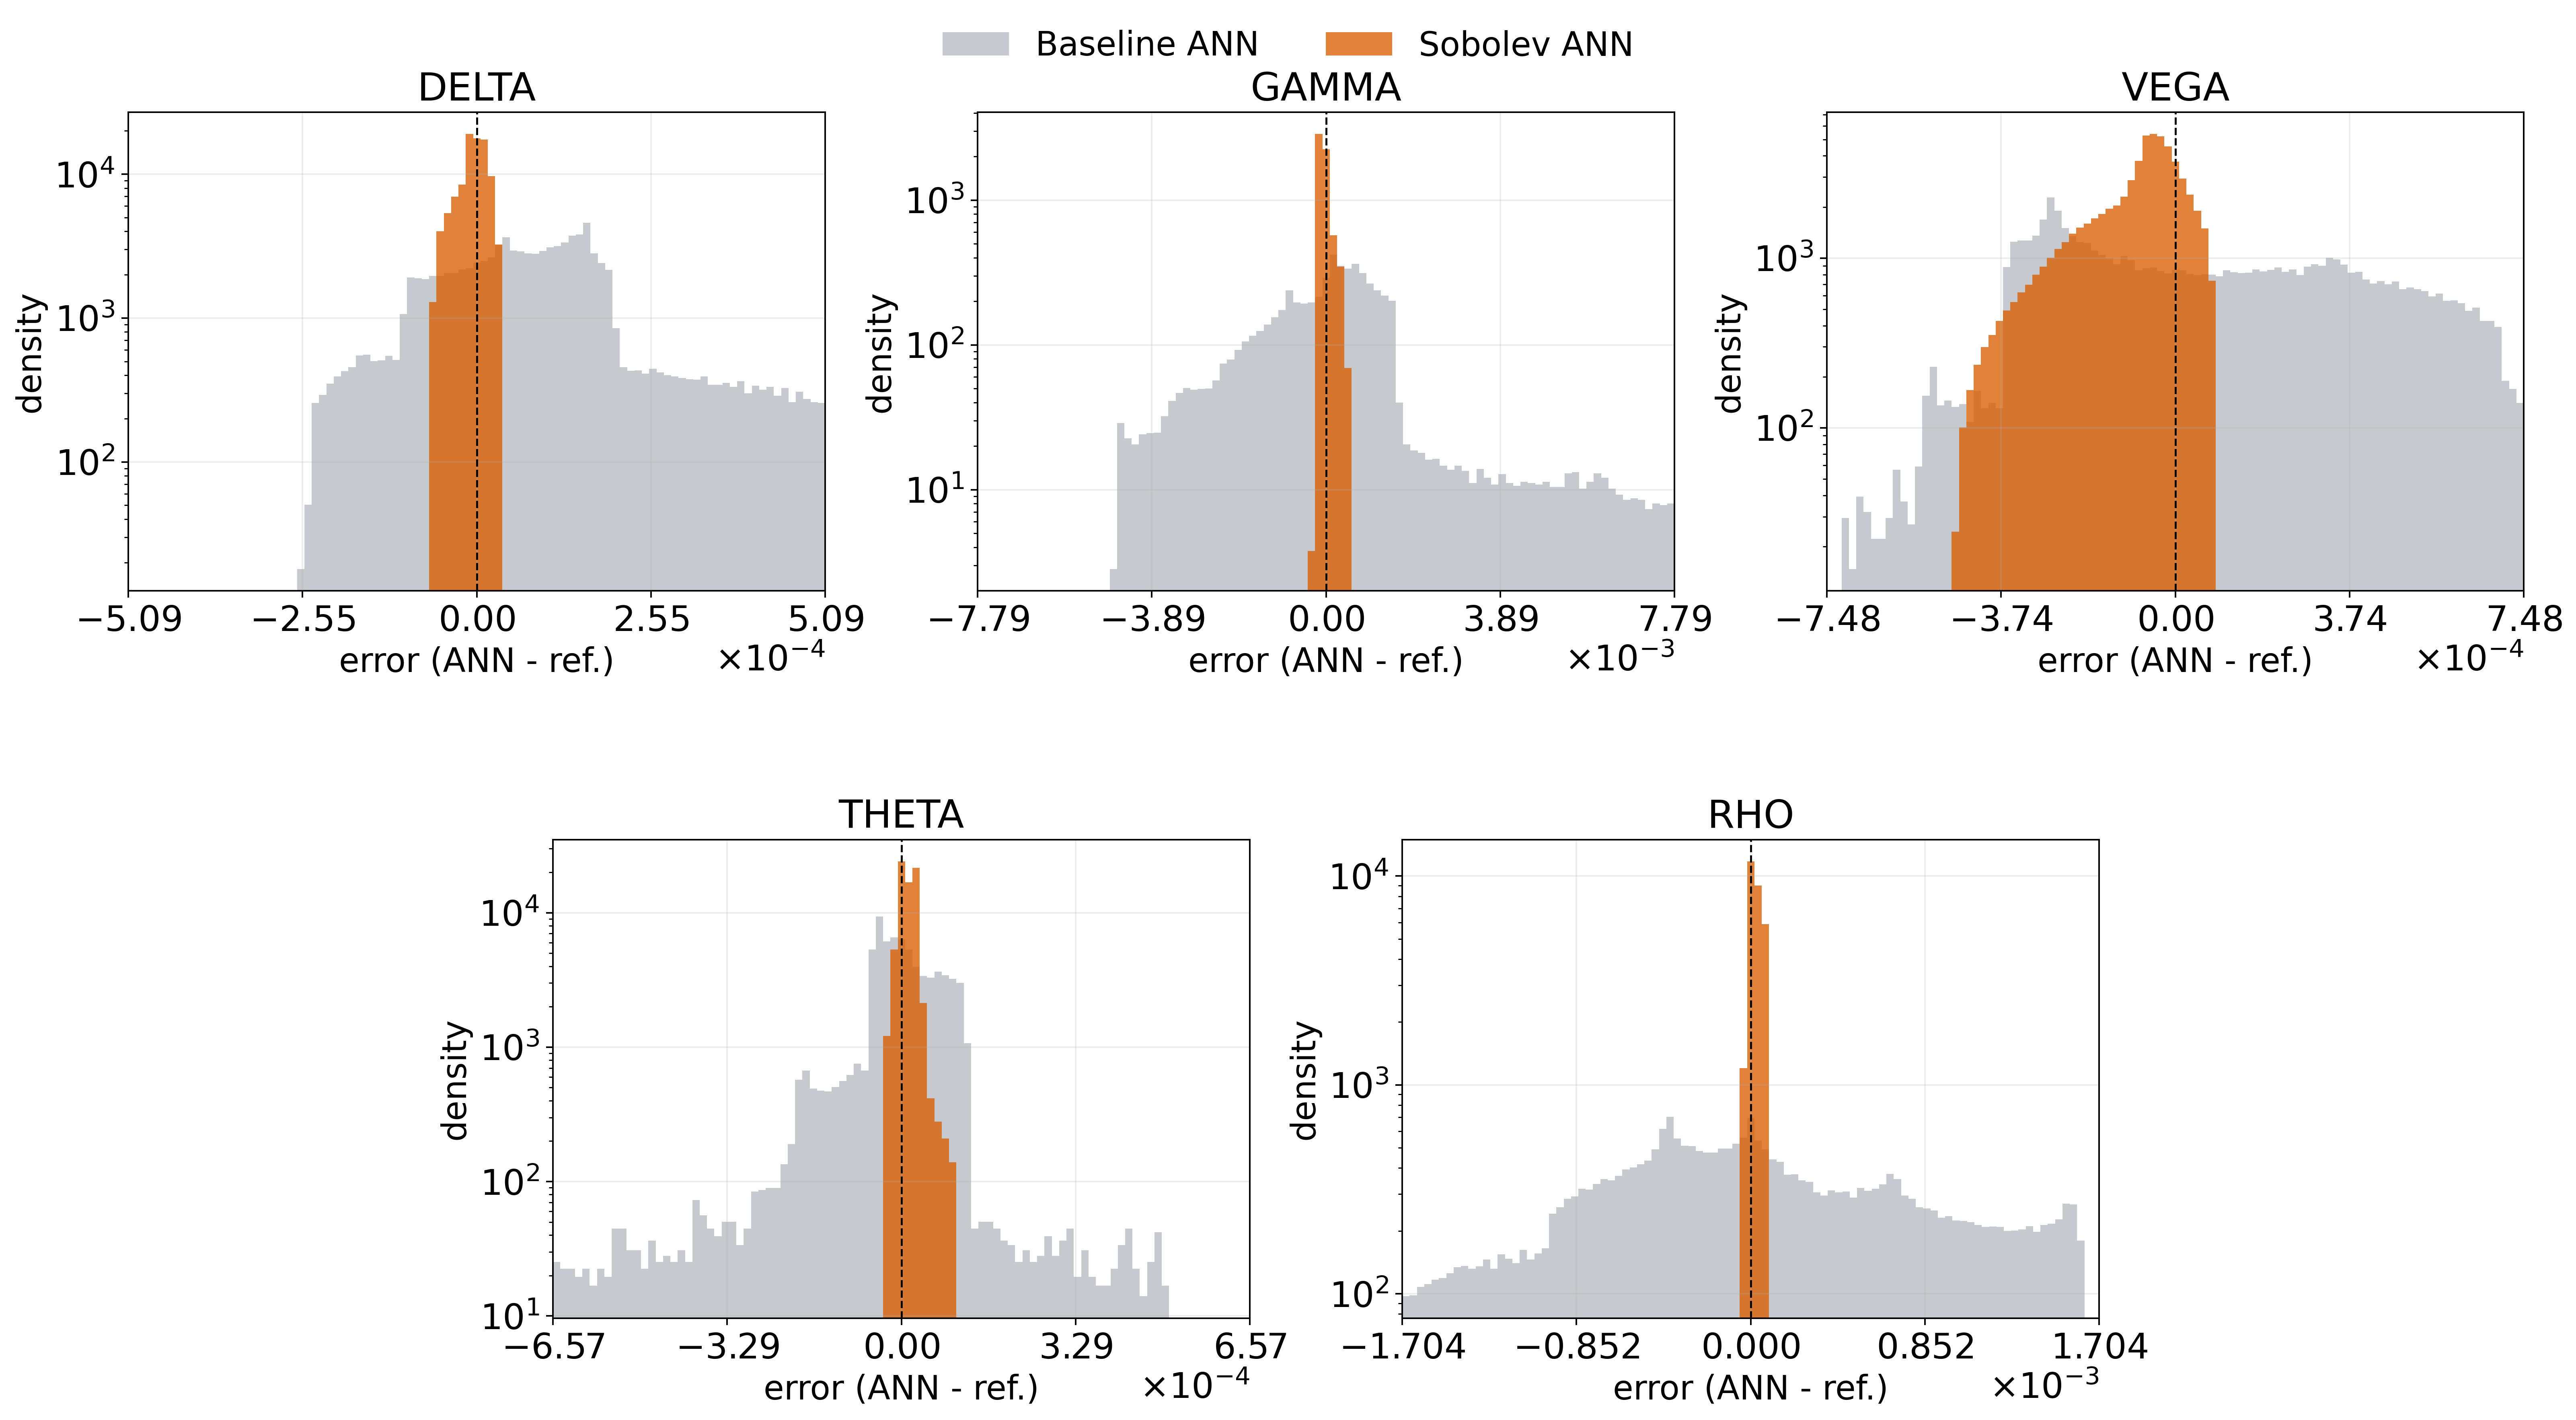
\includegraphics[width=\linewidth,height=0.73\textheight,keepaspectratio]{nn/ann_iv_baseline_vs_sobolev_error_hist_overlay_logy_5greeks.png}

  \vspace{1mm}
  \begin{itemize}
    \item Sobolev training narrows the error distributions for Delta, Gamma, Theta, and Rho.
    \item Vega also improves, although with a smaller separation between variants.
  \end{itemize}
\end{frame}

\begin{frame}{Sobolev improves ANN Greeks across the grid}
  \centering
  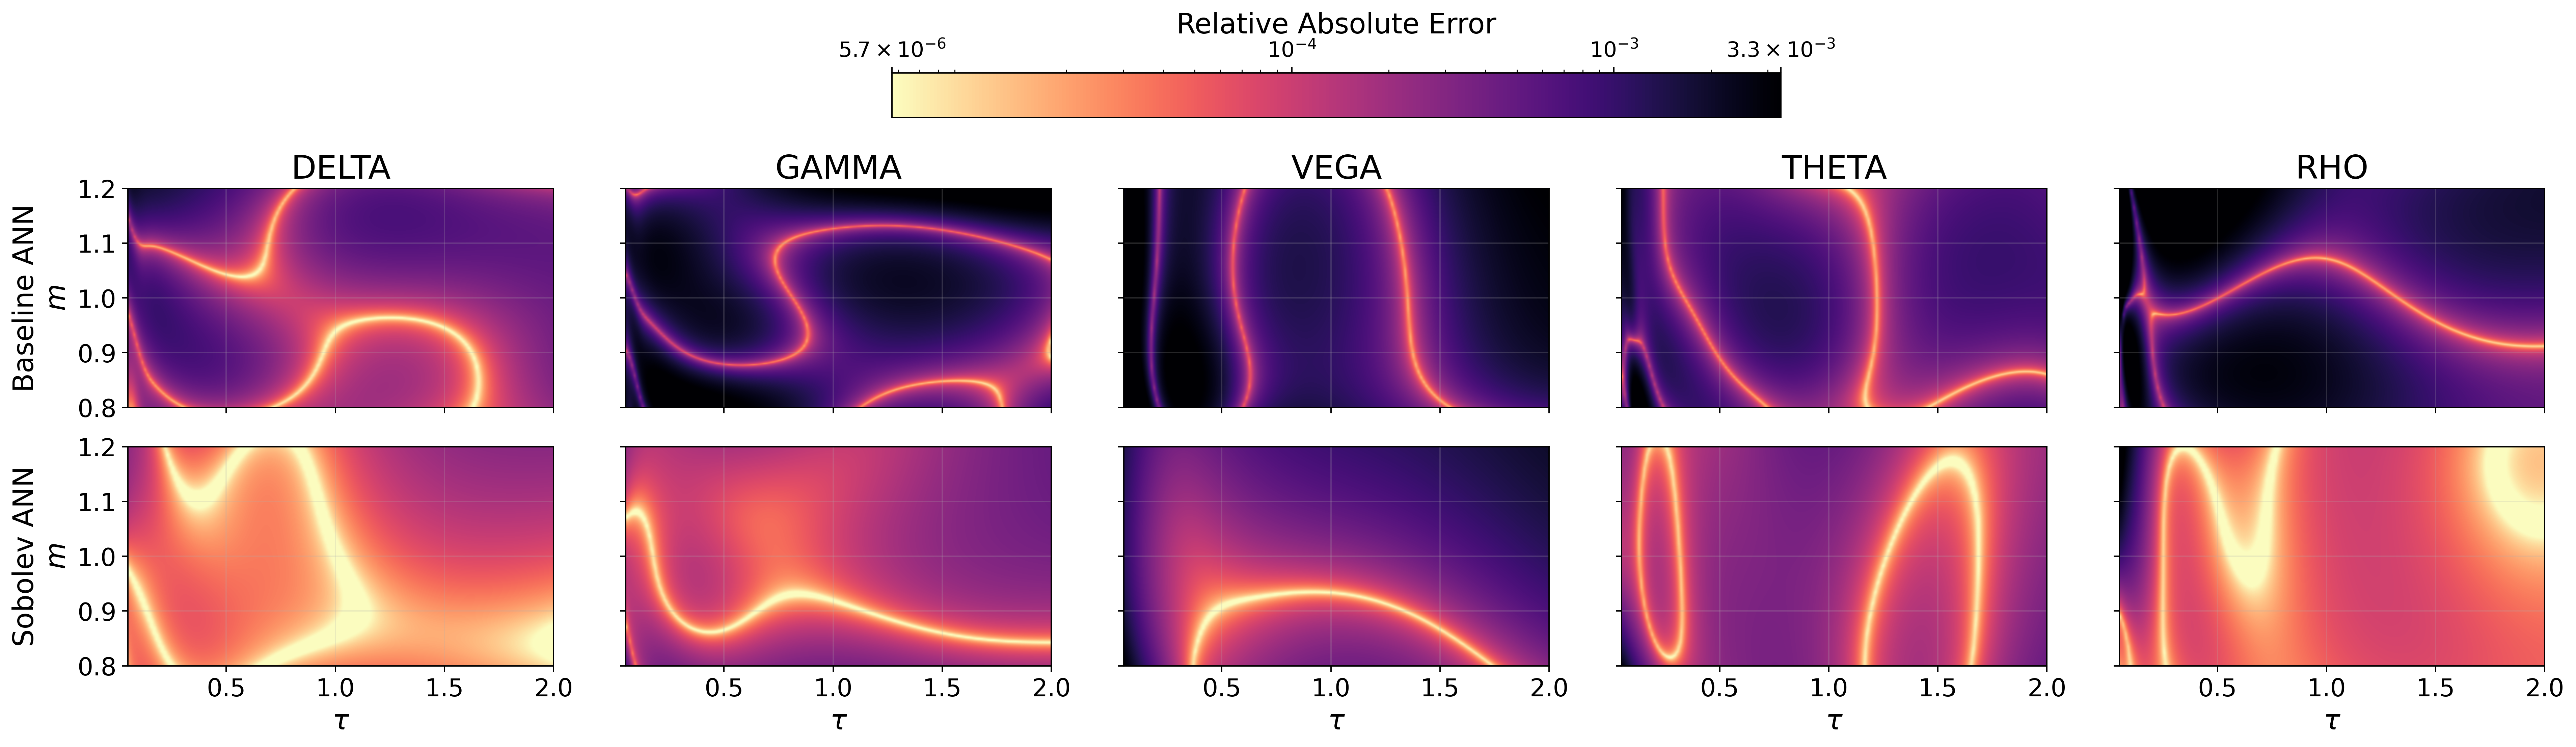
\includegraphics[width=\linewidth,height=0.76\textheight,keepaspectratio]{ann_sobolev_greek_rel_error_maps_landscape.png}

  \vspace{1mm}
  \begin{center}
    \scriptsize
    Greek RMSE ratios: Delta \(7.0\times\), Gamma \(12.7\times\), Vega \(2.2\times\), Theta \(5.0\times\), Rho \(20.8\times\).
  \end{center}
\end{frame}

\begin{frame}{The Sobolev IV surrogate gives tighter CaNN residuals}
  \begin{columns}[T,onlytextwidth]
    \begin{column}{0.50\textwidth}
      \centering
      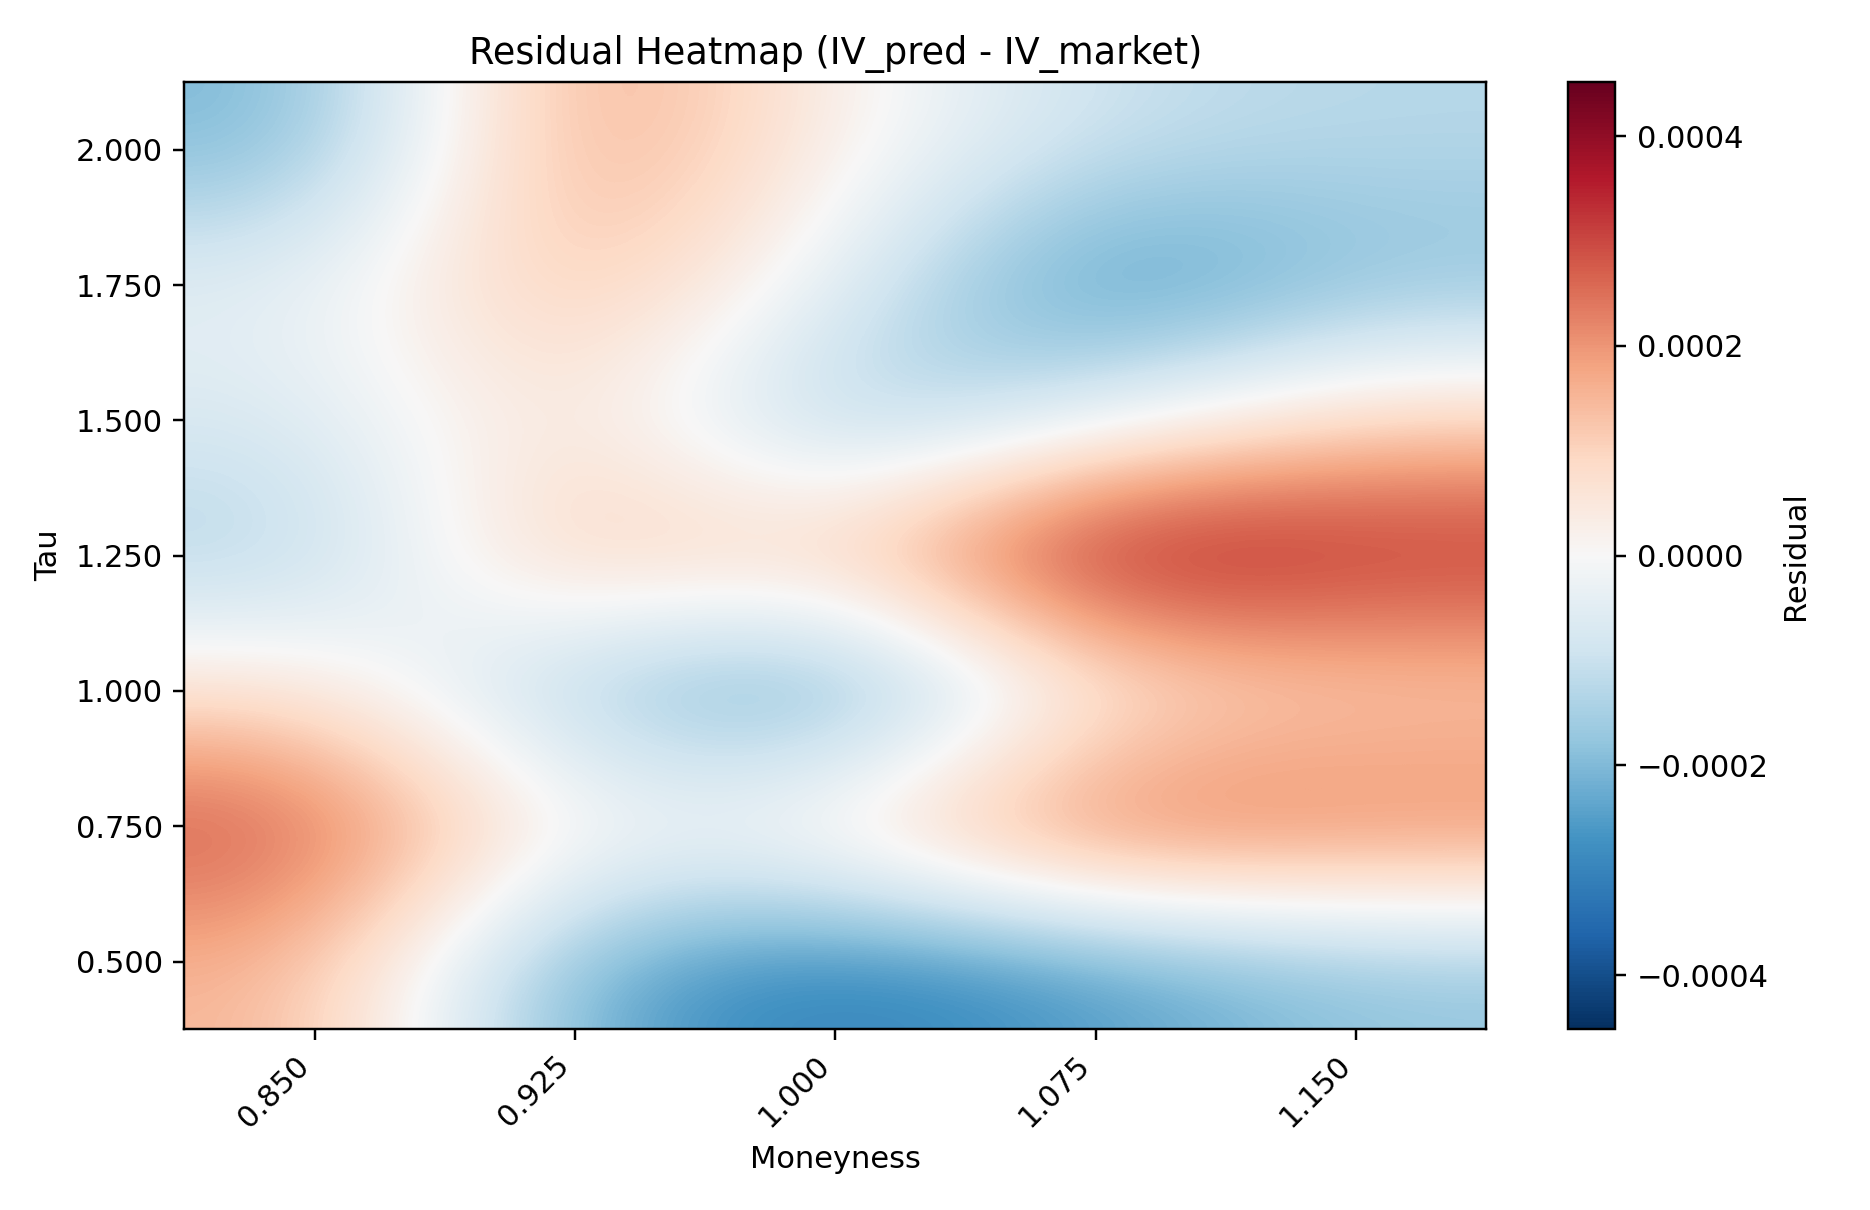
\includegraphics[width=\linewidth,height=0.67\textheight,keepaspectratio]{cann/cann_residual_heatmap_m_tau_l2_reg_smooth.png}
    \end{column}
    \begin{column}{0.46\textwidth}
      \centering
      \resizebox{\linewidth}{!}{%
      \begin{tabular}{lccc}
        \toprule
        Forward model & MSE & RMSE & \(\max |e|\) \\
        \midrule
        ANN baseline & \(7.43\cdot10^{-10}\) & \(2.73\cdot10^{-5}\) & \(6.79\cdot10^{-5}\) \\
        ANN Sobolev & \(3.69\cdot10^{-11}\) & \(6.08\cdot10^{-6}\) & \(1.36\cdot10^{-5}\) \\
        Liu et al. & \(\sim10^{-8}\) & -- & -- \\
        \bottomrule
      \end{tabular}}

      \vspace{6mm}
      \begin{itemize}
        \item Calibration is performed on the replicated \(35\)-quote Liu grid.
        \item The Sobolev forward surrogate gives the tightest IV residuals.
        \item Parameter recovery improves for four of the five Heston parameters relative to the baseline CaNN.
      \end{itemize}
    \end{column}
  \end{columns}
\end{frame}

\begin{frame}{The baseline PINN is strongest as a pricing model}
  \begin{columns}[T,onlytextwidth]
    \begin{column}{0.70\textwidth}
      \centering
      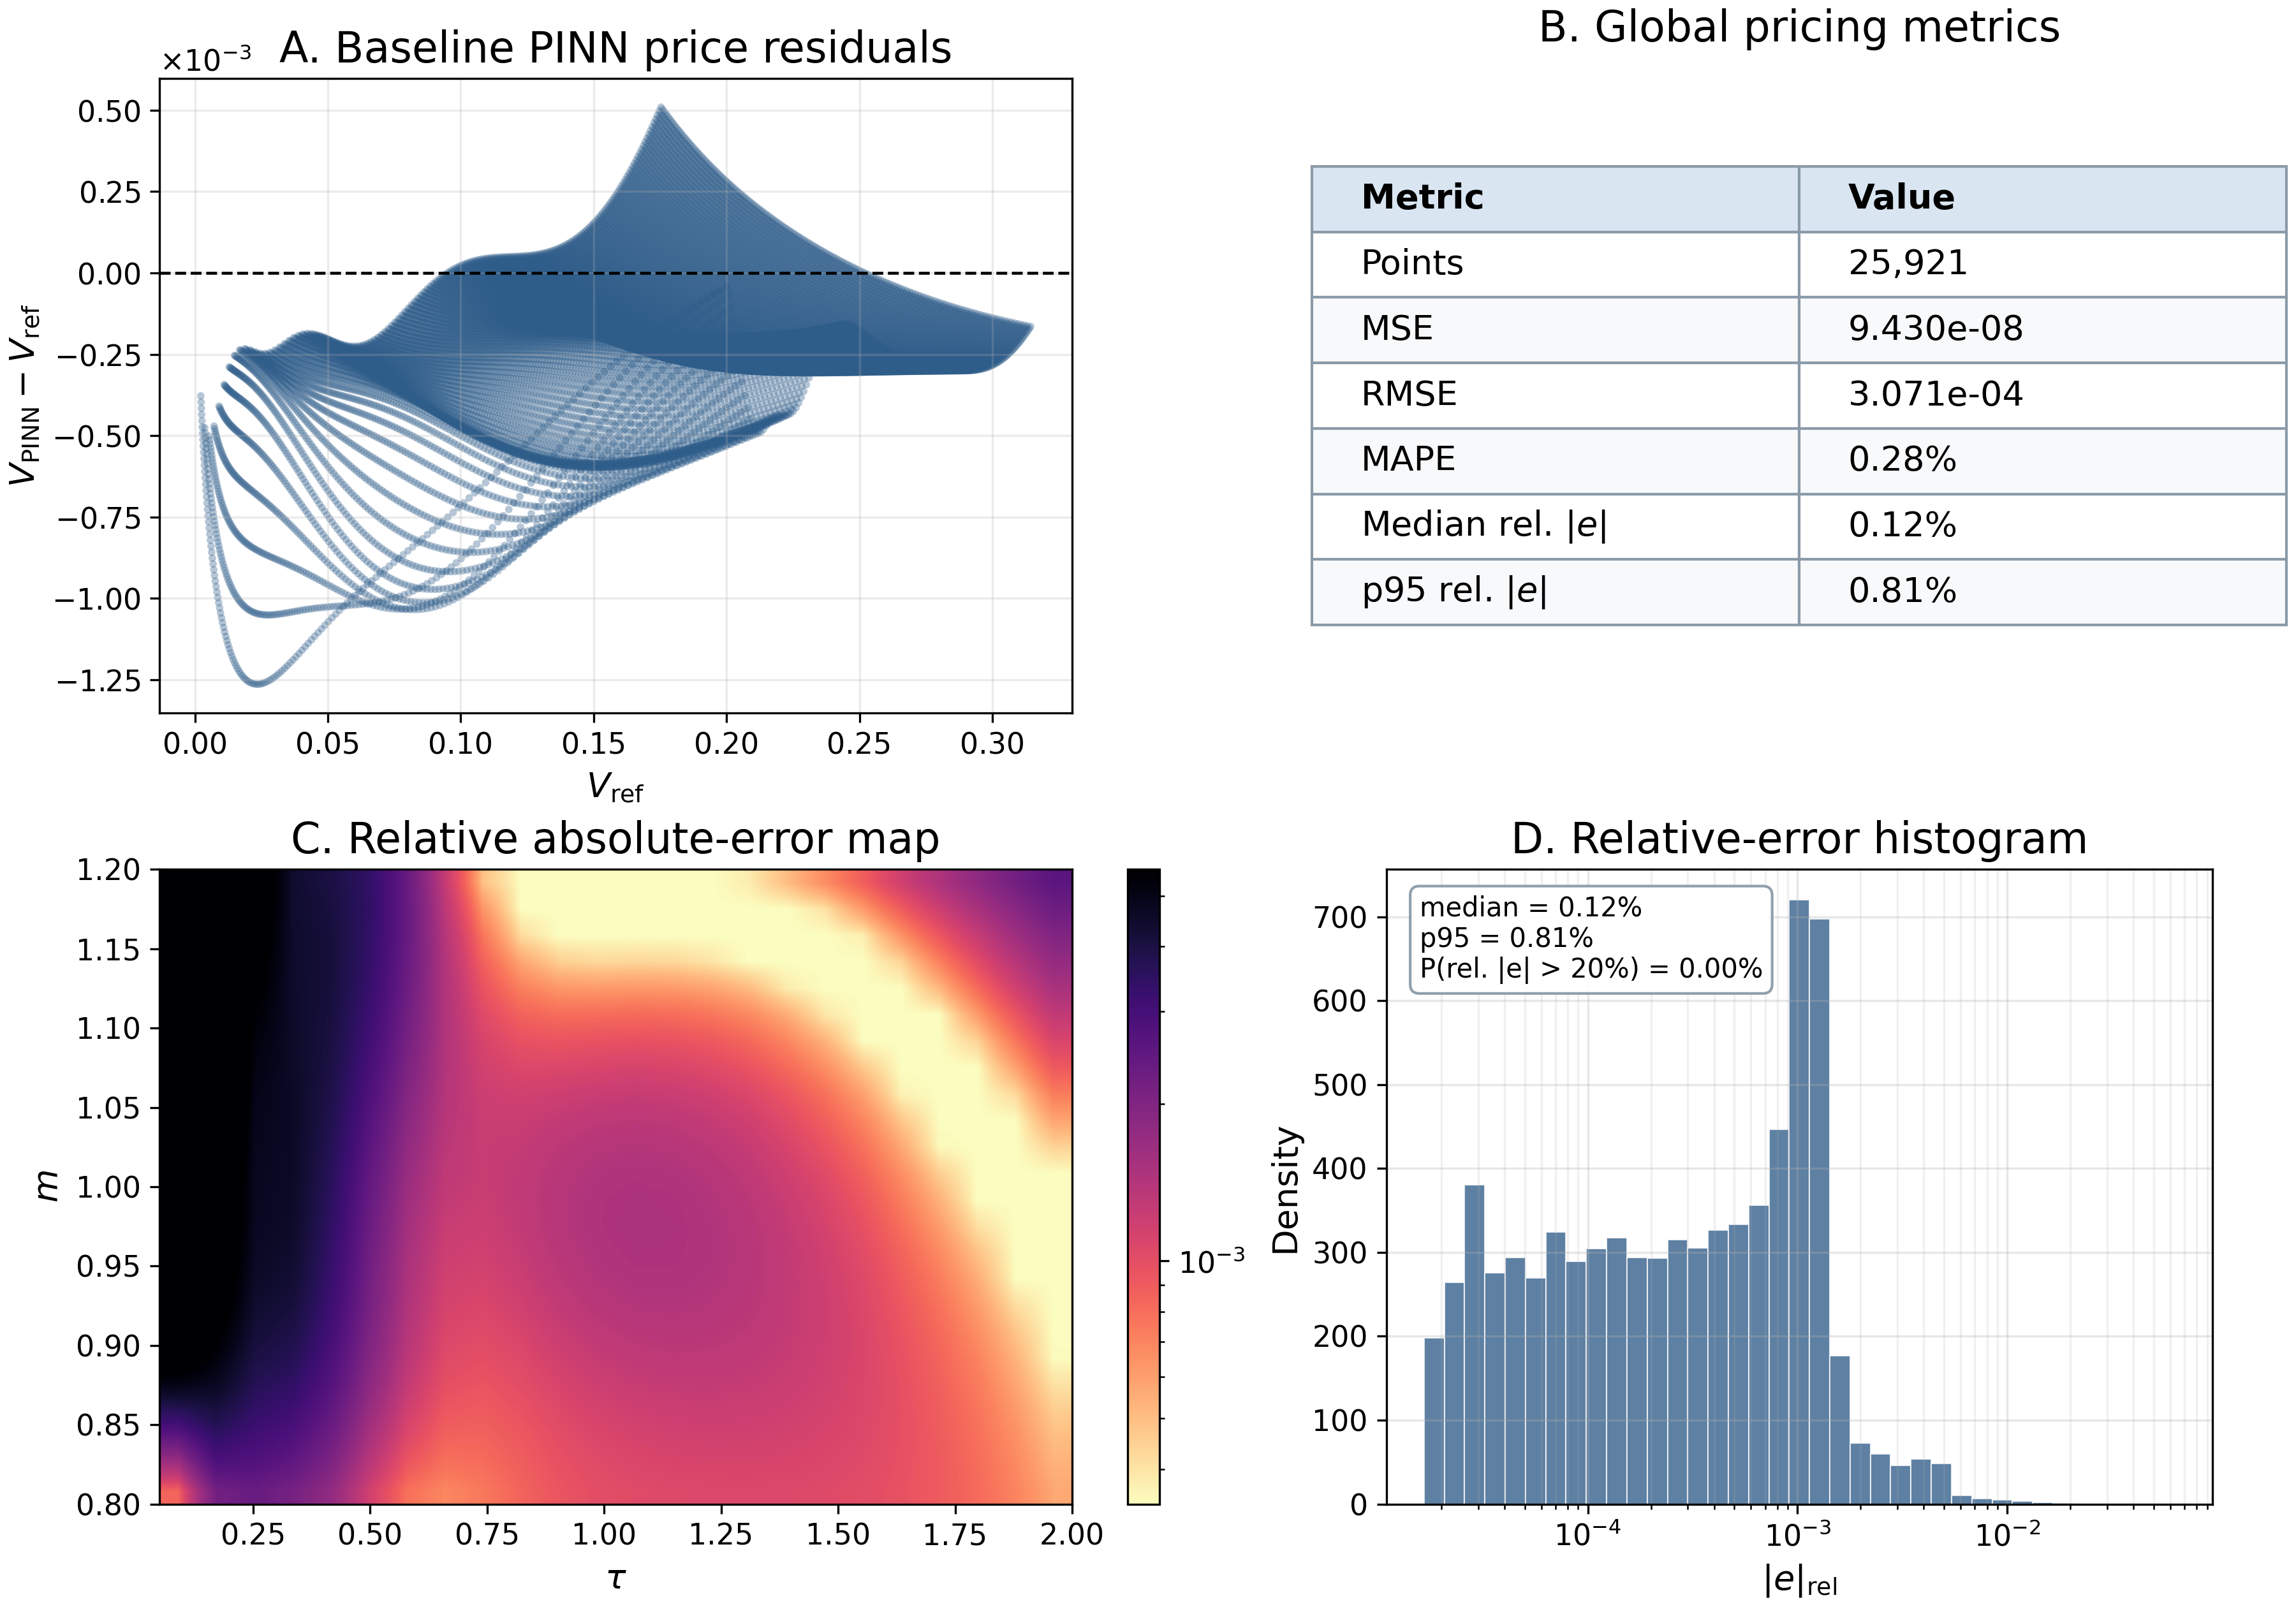
\includegraphics[width=\linewidth,height=0.78\textheight,keepaspectratio]{pinn/pricing/pricing_benchmark_composite.png}
    \end{column}
    \begin{column}{0.26\textwidth}
      \begin{itemize}
        \item Fixed grid:
        \[
          n=25{,}921.
        \]
        \item Price RMSE:
        \[
          3.07\cdot10^{-4}.
        \]
        \item MAPE:
        \[
          0.28\%.
        \]
      \end{itemize}
    \end{column}
  \end{columns}
\end{frame}

\begin{frame}{Sobolev improves PINN Greeks under a different regime}
  \centering
  \small
  \begin{tabular}{lccc}
    \toprule
    Greek & PINN baseline RMSE & PINN Sobolev RMSE & Ratio \\
    \midrule
    Delta & \(3.33\cdot10^{-2}\) & \(3.51\cdot10^{-4}\) & \(94.9\times\) \\
    Gamma & \(3.85\cdot10^{-1}\) & \(8.94\cdot10^{-3}\) & \(43.1\times\) \\
    Vega  & \(6.55\cdot10^{-2}\) & \(3.17\cdot10^{-3}\) & \(20.7\times\) \\
    Theta & \(4.82\cdot10^{-3}\) & \(5.30\cdot10^{-4}\) & \(9.1\times\) \\
    Rho   & \(8.37\cdot10^{-2}\) & \(1.43\cdot10^{-3}\) & \(58.5\times\) \\
    \bottomrule
  \end{tabular}

  \vspace{6mm}
  \begin{itemize}
    \item Sobolev terms strongly improve full-grid Greek diagnostics.
    \item The interpretation is not a uniform model improvement: derivative labels change the information regime.
    \item Greek throughput changes from \(9.48\cdot10^3\) to \(8.60\cdot10^3\) points/s.
  \end{itemize}
\end{frame}

\begin{frame}{Short maturities remain the hardest PINN region}
  \centering
  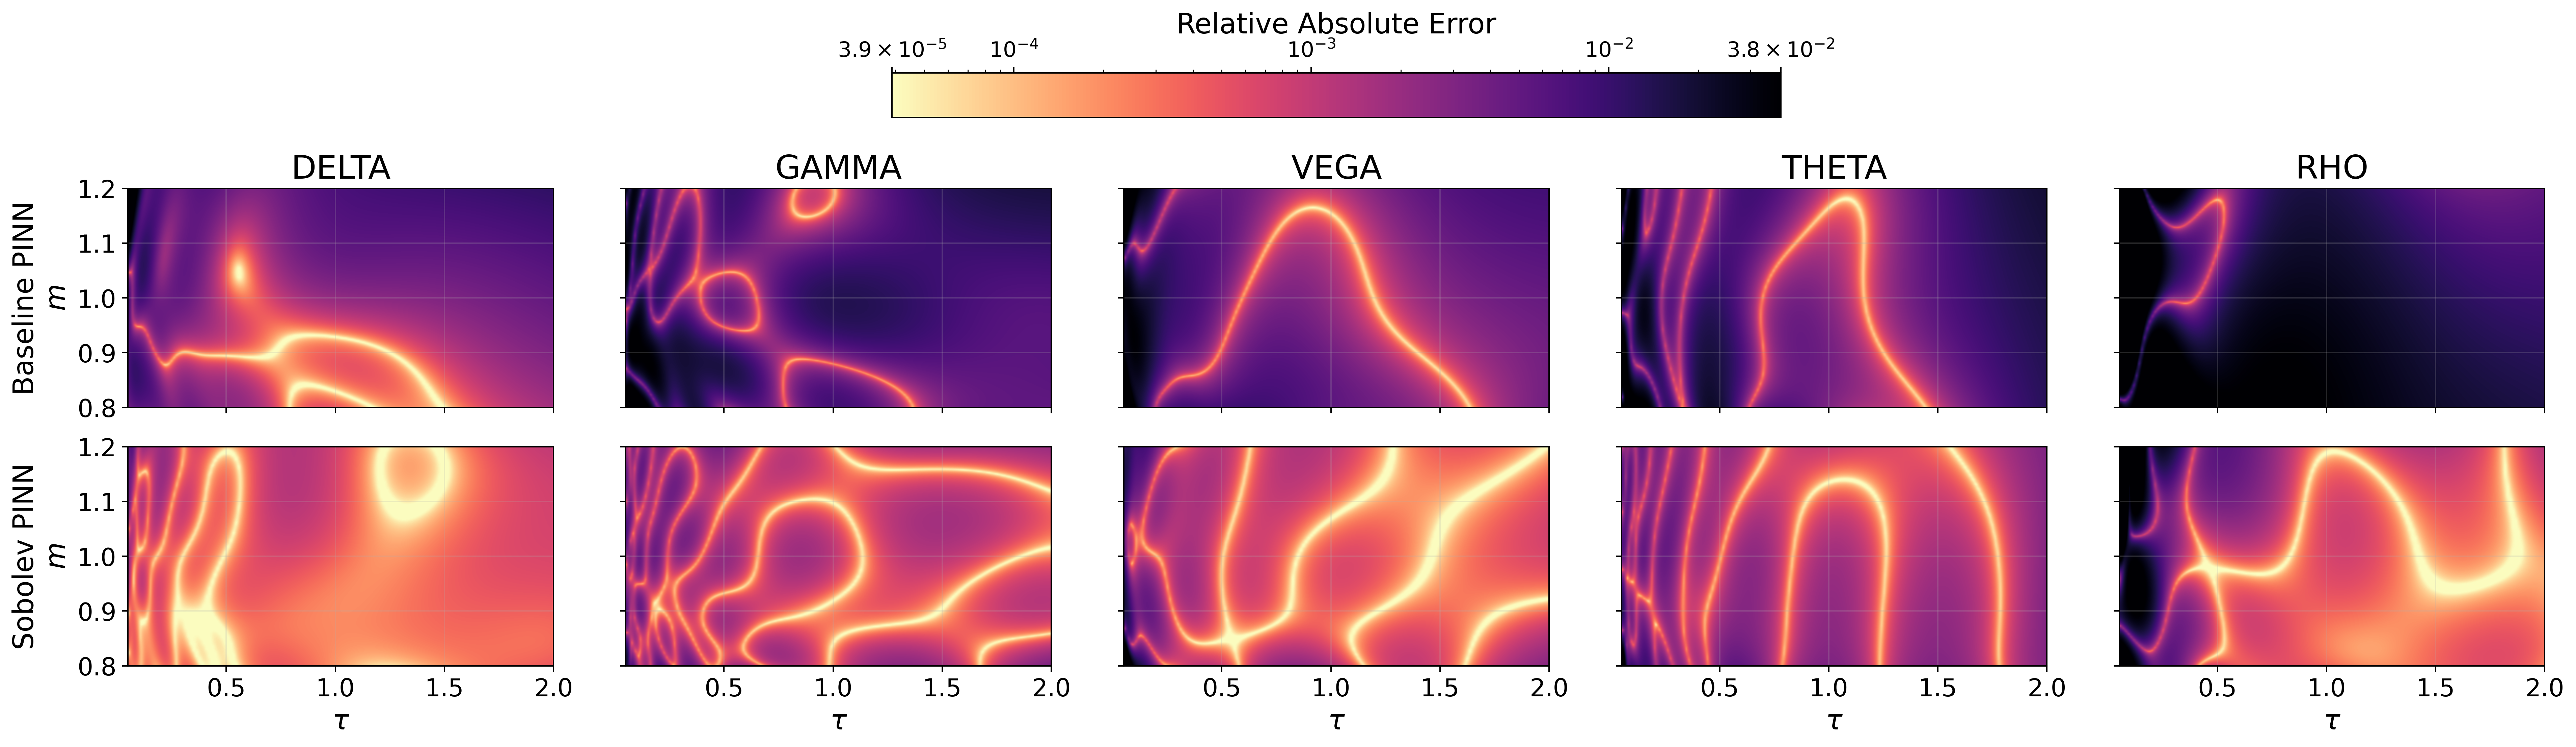
\includegraphics[width=\linewidth,height=0.76\textheight,keepaspectratio]{pinn_sobolev_greek_rel_error_maps_landscape.png}

  \vspace{1mm}
  \begin{itemize}
    \item Sobolev reduces global errors, but the short-maturity region remains structured.
    \item This motivates a separate local diagnostic around the payoff kink.
  \end{itemize}
\end{frame}

\begin{frame}{ACV targets the short-maturity ATM hard region}
  \centering
  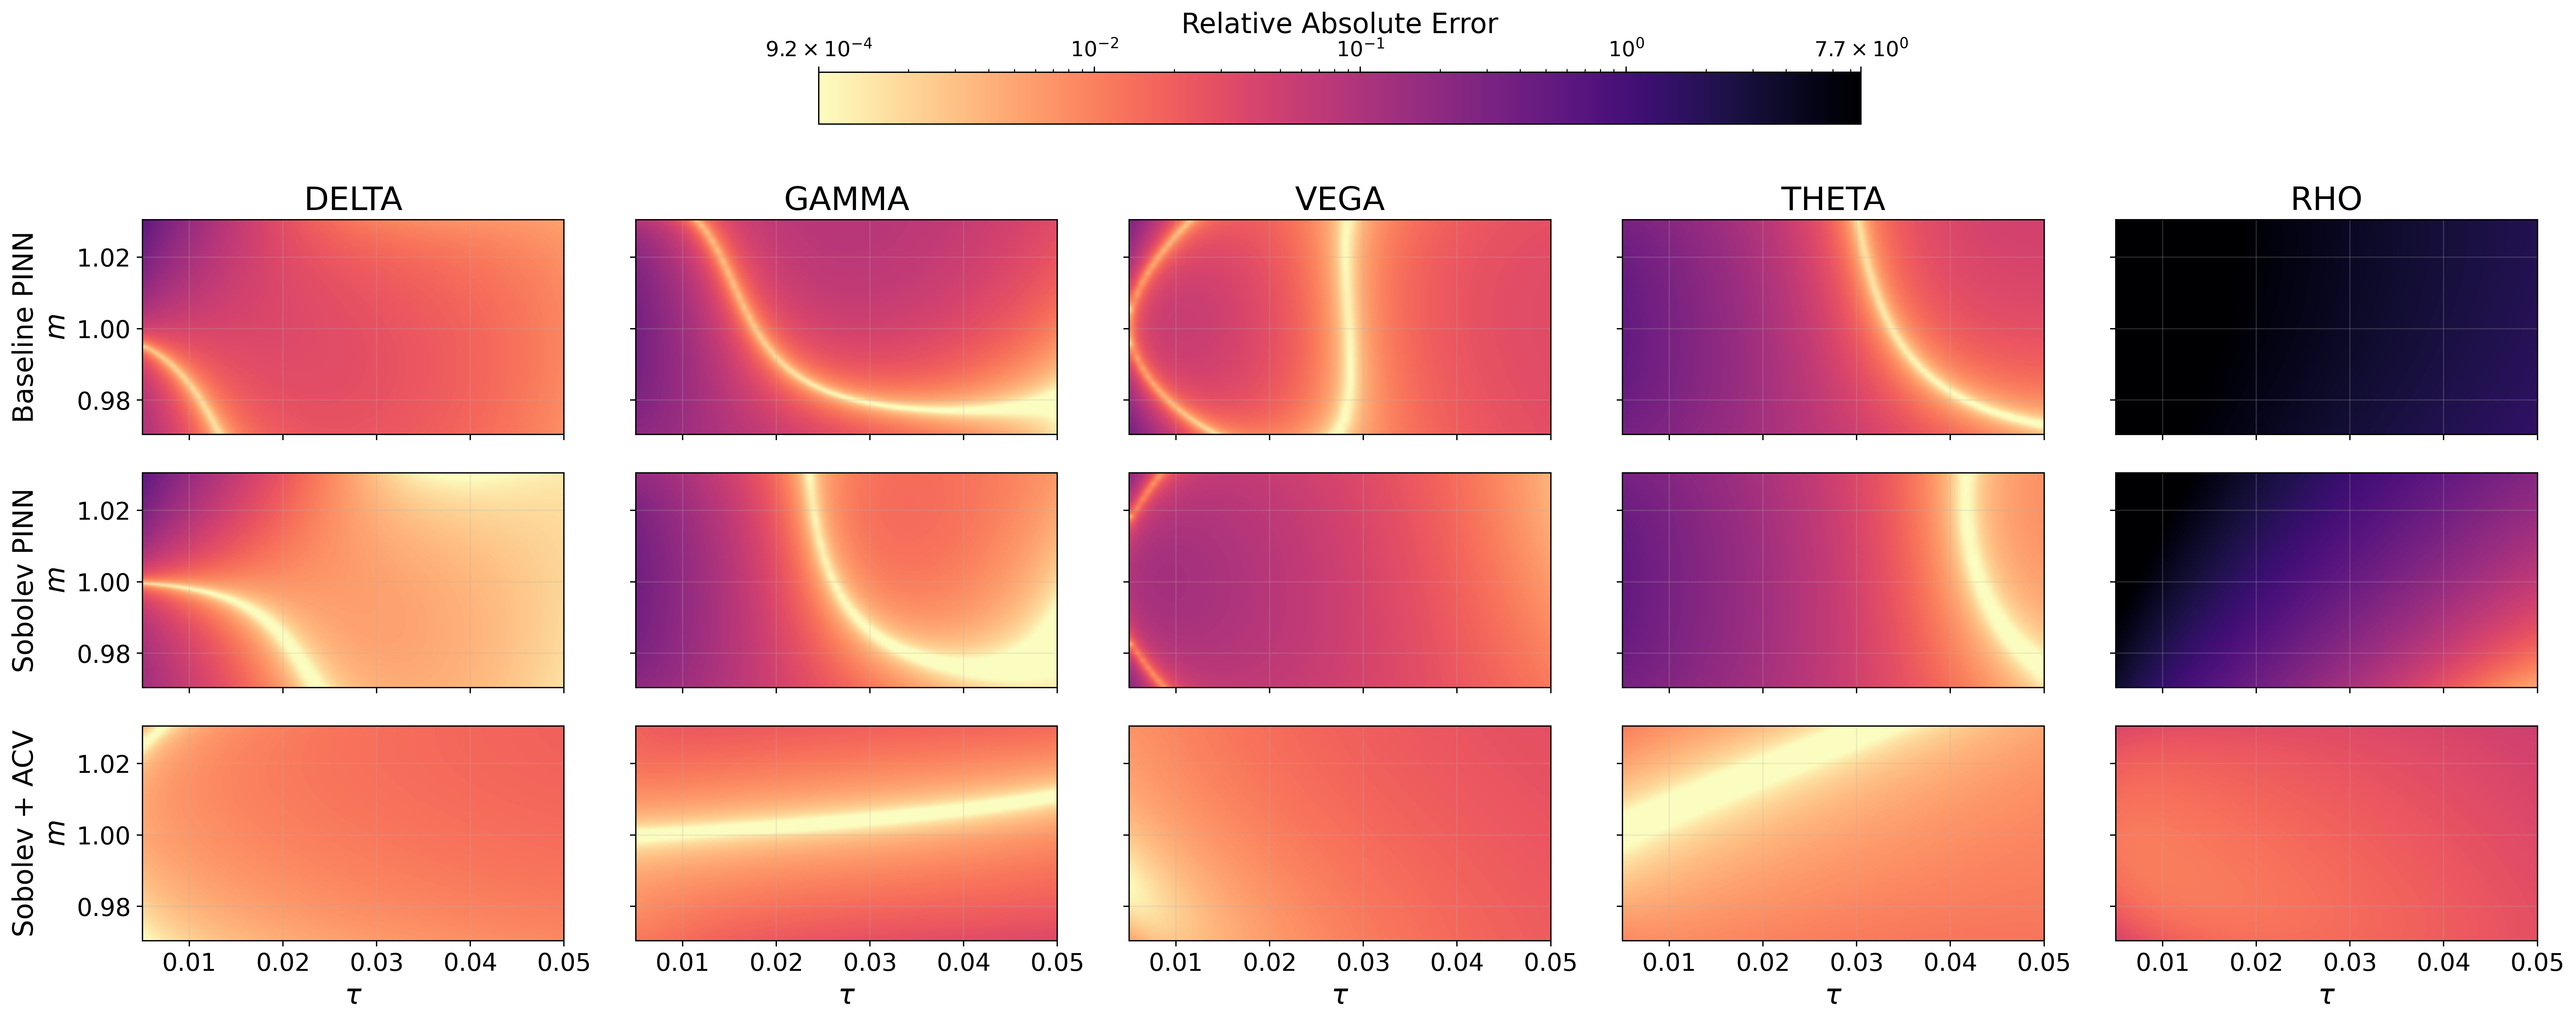
\includegraphics[width=\linewidth,height=0.77\textheight,keepaspectratio]{pinn_sobolev_acv_greek_rel_error_maps_landscape.png}

  \vspace{1mm}
  \begin{center}
    \scriptsize
    Hard-region grid: \(m\in[0.9704,1.0305]\), \(\tau\in[0.005,0.05]\).
  \end{center}
\end{frame}

\begin{frame}{Neural evaluators are faster after training}
  \centering
  \begin{tabular}{lrr}
    \toprule
    Component & Throughput & Unit \\
    \midrule
    ANN evaluator & \(8.43\cdot10^{5}\) & IV evaluations/s \\
    PINN pricing & \(4.91\cdot10^{5}\) & price points/s \\
    COS repeated pricing & \(8.736\cdot10^{1}\) & price points/s \\
    PINN Greek baseline & \(9.48\cdot10^{3}\) & Greek points/s \\
    PINN Greek Sobolev & \(8.60\cdot10^{3}\) & Greek points/s \\
    \bottomrule
  \end{tabular}

  \vspace{7mm}
  \begin{itemize}
    \item The speed advantage appears after training, in repeated evaluation mode.
    \item The comparison is not used to rank all models globally; it quantifies the computational role of each branch.
  \end{itemize}
\end{frame}

\section{Conclusions}

\begin{frame}{Main takeaways}
  \begin{enumerate}
    \item Placeholder takeaway on numerical accuracy.
    \item Placeholder takeaway on computational efficiency.
    \item Placeholder takeaway on calibration usefulness.
    \item Placeholder takeaway on limitations and robustness.
  \end{enumerate}
\end{frame}

\begin{frame}{Future work}
  \begin{itemize}
    \item Extend the model family or market-data coverage.
    \item Improve no-arbitrage and Greek consistency constraints.
    \item Strengthen out-of-domain diagnostics.
    \item Package the workflow for reproducible pricing and calibration experiments.
  \end{itemize}
\end{frame}

\begin{frame}
  \centering
  {\Huge Thank you}

  \vspace{1cm}
  {\Large Questions}
\end{frame}


\appendix

\begin{frame}[plain]
  \centering
  \vfill
  {\Huge EXTRAS}
  \vfill
\end{frame}

\begin{frame}{ANN Sobolev value surfaces}
  \centering
  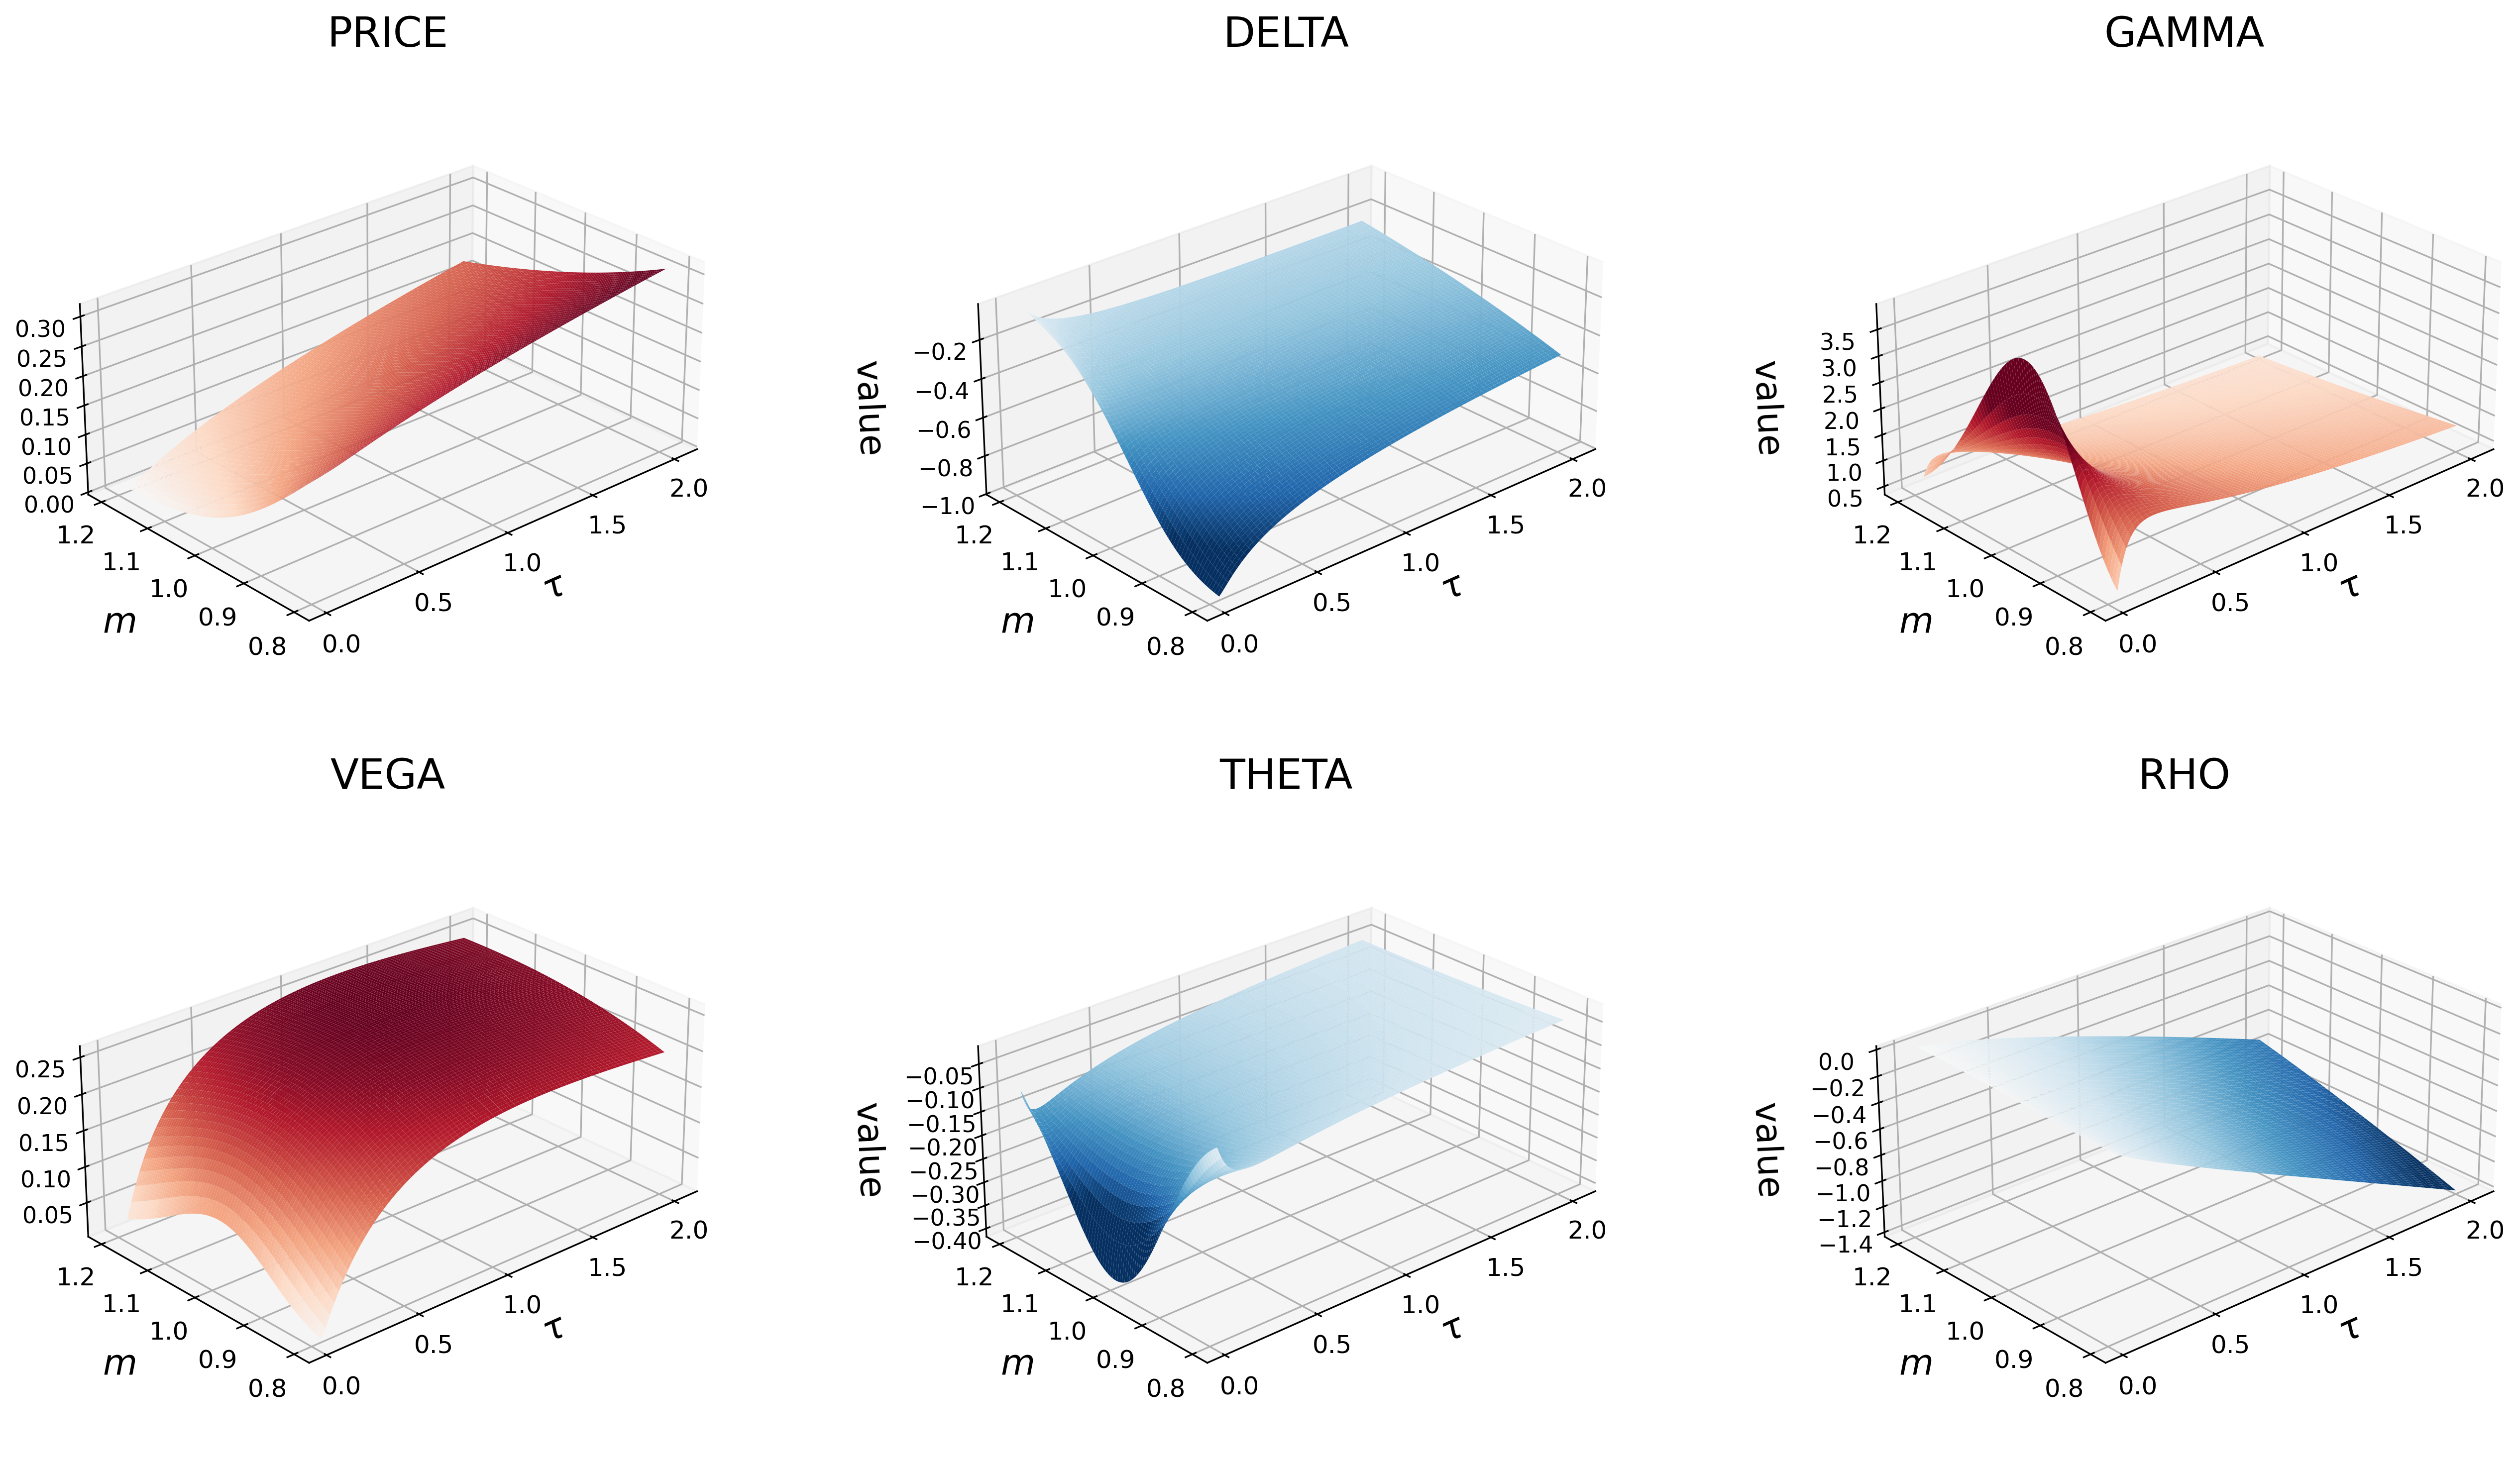
\includegraphics[width=\linewidth,height=0.84\textheight,keepaspectratio]{nn/ann_sobolev_price_greek_value_surfaces_3d.png}
\end{frame}

\begin{frame}{Kink-region value surfaces}
  \centering
  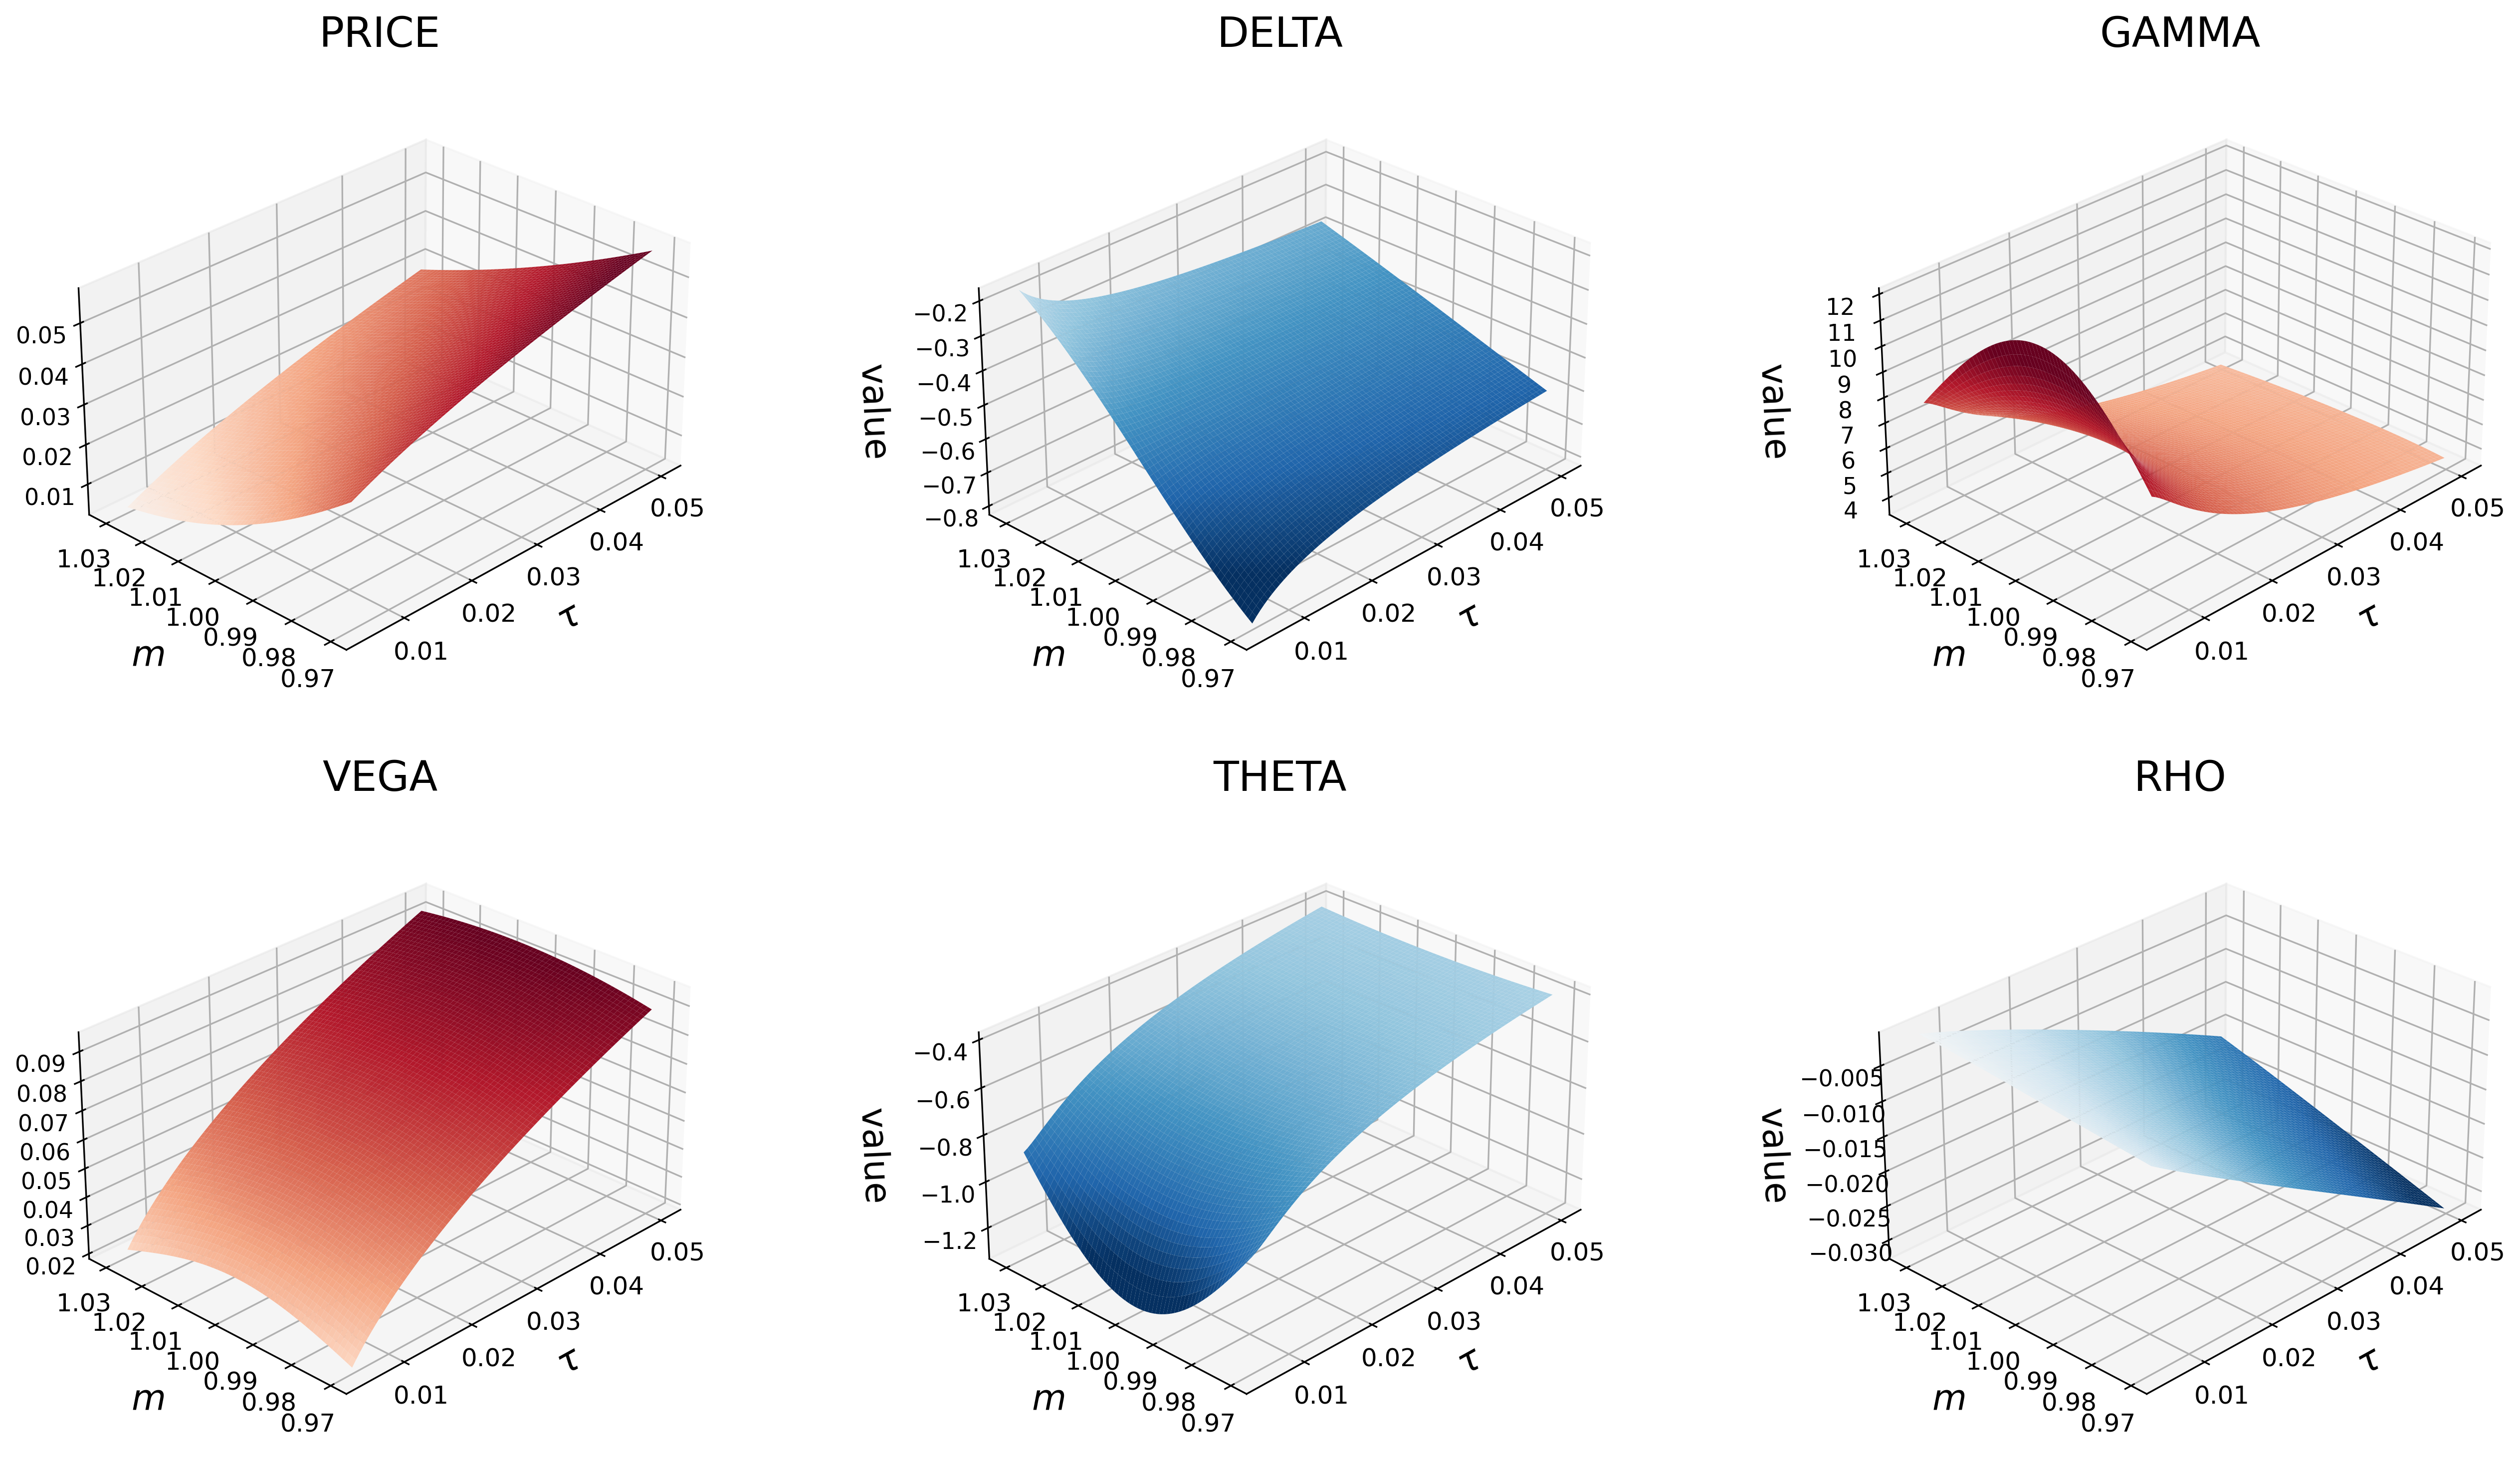
\includegraphics[width=\linewidth,height=0.84\textheight,keepaspectratio]{pinn/greeks/pinn_sobolev_acv_kink_price_greek_value_surfaces_3d.png}
\end{frame}


\end{document}
